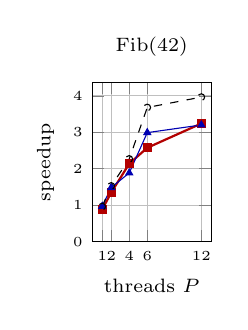
\begin{tikzpicture}
\begin{axis}[width=0.255\textwidth,height=3.6cm,title={\scriptsize Fib(42)},xlabel={\scriptsize threads $P$},ylabel={\scriptsize speedup},
 xtick={1,2,4,6,12},tick label style={font=\tiny},grid=major,ymin=0]
\addplot[red!70!black,thick,mark=square*,mark size=1.2pt] coordinates {(1,0.884) (2,1.347) (4,2.139) (6,2.576) (12,3.243)};
\addplot[blue!70!black,mark=triangle*,mark size=1.4pt] coordinates {(1,0.970) (2,1.485) (4,1.886) (6,2.992) (12,3.203)};
\addplot[black,dashed,mark=o,mark size=1.2pt] coordinates {(1,0.962) (2,1.528) (4,2.270) (6,3.683) (12,3.968)};
\end{axis}
\end{tikzpicture}\hfill
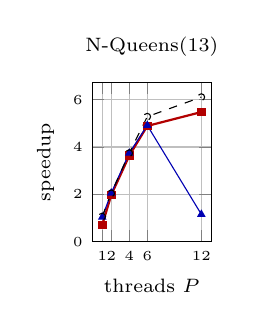
\begin{tikzpicture}
\begin{axis}[width=0.255\textwidth,height=3.6cm,title={\scriptsize N-Queens(13)},xlabel={\scriptsize threads $P$},ylabel={\scriptsize speedup},
 xtick={1,2,4,6,12},tick label style={font=\tiny},grid=major,ymin=0]
\addplot[red!70!black,thick,mark=square*,mark size=1.2pt] coordinates {(1,0.703) (2,1.968) (4,3.631) (6,4.888) (12,5.476)};
\addplot[blue!70!black,mark=triangle*,mark size=1.4pt] coordinates {(1,1.032) (2,2.051) (4,3.737) (6,4.914) (12,1.153)};
\addplot[black,dashed,mark=o,mark size=1.2pt] coordinates {(1,1.062) (2,2.042) (4,3.741) (6,5.281) (12,6.108)};
\end{axis}
\end{tikzpicture}\hfill
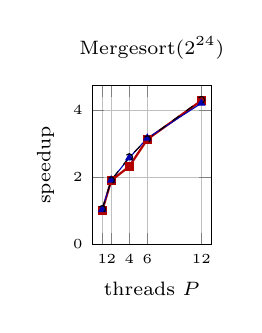
\begin{tikzpicture}
\begin{axis}[width=0.255\textwidth,height=3.6cm,title={\scriptsize Mergesort($2^{24}$)},xlabel={\scriptsize threads $P$},ylabel={\scriptsize speedup},
 xtick={1,2,4,6,12},tick label style={font=\tiny},grid=major,ymin=0]
\addplot[red!70!black,thick,mark=square*,mark size=1.2pt] coordinates {(1,1.004) (2,1.906) (4,2.326) (6,3.136) (12,4.293)};
\addplot[blue!70!black,mark=triangle*,mark size=1.4pt] coordinates {(1,1.040) (2,1.918) (4,2.581) (6,3.171) (12,4.215)};
\addplot[black,dashed,mark=o,mark size=1.2pt] coordinates {(1,1.058) (2,1.915) (4,2.606) (6,3.142) (12,4.316)};
\end{axis}
\end{tikzpicture}\hfill
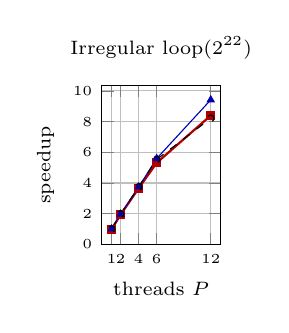
\begin{tikzpicture}
\begin{axis}[width=0.255\textwidth,height=3.6cm,title={\scriptsize Irregular loop($2^{22}$)},xlabel={\scriptsize threads $P$},ylabel={\scriptsize speedup},
 xtick={1,2,4,6,12},tick label style={font=\tiny},grid=major,ymin=0]
\addplot[red!70!black,thick,mark=square*,mark size=1.2pt] coordinates {(1,0.993) (2,1.935) (4,3.656) (6,5.311) (12,8.395)};
\addplot[blue!70!black,mark=triangle*,mark size=1.4pt] coordinates {(1,1.000) (2,1.970) (4,3.736) (6,5.592) (12,9.416)};
\addplot[black,dashed,mark=o,mark size=1.2pt] coordinates {(1,1.003) (2,1.977) (4,3.744) (6,5.532) (12,8.211)};
\end{axis}
\end{tikzpicture}
